\documentclass[conference]{IEEEtran}

% ── Packages ──────────────────────────────────────────────────────────────────
\usepackage{cite}
\usepackage{amsmath,amssymb,amsfonts}
\usepackage{algorithmic}
\usepackage{graphicx}
\usepackage{textcomp}
\usepackage{xcolor}
\usepackage{hyperref}
\usepackage{booktabs}
\usepackage{subfig}
\usepackage{tikz}
\usepackage{pgfplots}
\pgfplotsset{compat=1.18}
\usetikzlibrary{arrows.meta,positioning,shapes.geometric,fit,backgrounds,calc}

% ── Macros ────────────────────────────────────────────────────────────────────
\newcommand{\vd}{\mathbf{v}_d}
\newcommand{\veeEE}{\mathbf{v}_{ee}}
\newcommand{\nn}{\mathbf{n}}
\newcommand{\pp}{\mathbf{p}}
\newcommand{\qq}{\mathbf{q}}
\newcommand{\JJ}{\mathbf{J}}
\newcommand{\DD}{\mathbf{D}}
\newcommand{\Fc}{\mathbf{F}_{cart}}
\newcommand{\tauv}{\boldsymbol{\tau}}
\newcommand{\R}{\mathbb{R}}

% ─────────────────────────────────────────────────────────────────────────────
\begin{document}

\title{DS-Based Surface Polishing in Simulation:\\
A MuJoCo Reproduction of Passive Impedance Control\\
on a 3/8-Sphere Surface}

\author{
  \IEEEauthorblockN{Cindy Wu}
  \IEEEauthorblockA{
    \textit{Department of Mechanical Engineering and Applied Mechanics}\\
    University of Pennsylvania\\
    Philadelphia, PA, USA\\
    cindywuliwu2001@gmail.com
  }
}

\maketitle

% ─────────────────────────────────────────────────────────────────────────────
\begin{abstract}
We present a Python/MuJoCo simulation that reproduces the core ideas of
dynamical-systems (DS)-based contact tasks, originally implemented in C++/ROS
by Amanhoud \emph{et al.}~\cite{amanhoud2019} on a KUKA LWR IV+ manipulator.
The target scenario is a Franka Emika Panda robot polishing the outer surface of
a $3/8$-sphere ($R=0.15$~m) while maintaining a desired contact force of 5~N.
The control architecture combines a DS velocity field that blends a reaching
component with a tangential circular limit-cycle, and a passive DS impedance
controller (without tank energy) that maps the desired EE velocity to joint
torques via $\tauv = \JJ^T \DD(\vd - \veeEE) + \mathbf{g}(\qq)$.
Simulation results demonstrate successful approach, stable surface following,
and a repeatable circular polishing trajectory over the $3/8$-sphere surface.
We discuss the design choices, performance metrics, and the gap between
the idealized torque-controlled hardware and the simulated dynamics.
\end{abstract}

\begin{IEEEkeywords}
dynamical systems, impedance control, surface polishing, contact tasks,
MuJoCo, Franka Panda
\end{IEEEkeywords}

% =============================================================================
\section{Introduction}
\label{sec:intro}

Physical interaction between robots and their environment remains one of the
central challenges in manipulation. Unlike free-space motion, contact tasks
require simultaneous control of \emph{position} (staying on the surface) and
\emph{force} (applying the right pressure). Classical impedance
control~\cite{hogan1985} achieves a trade-off between the two by defining a
target mechanical impedance for the end-effector. However, the desired motion
trajectory must still be specified separately.

Dynamical Systems (DS) offer an elegant alternative: the robot's desired
velocity is encoded as a globally stable vector field rather than a
pre-computed path~\cite{khansari2014}. When combined with impedance control,
DS-based methods can handle variable contact geometry and
unexpected perturbations without replanning~\cite{amanhoud2019}.

Amanhoud \emph{et al.}~\cite{amanhoud2019} implemented such a system on a
KUKA LWR IV+ robot for circular surface polishing. Their approach uses a
passive DS impedance controller augmented with a tank-energy mechanism to
guarantee passivity during all phases. In this project, we reproduce the
core concepts in simulation—dropping the tank-energy term for simplicity—and
deploy the resulting controller on a Franka Emika Panda robot in
MuJoCo~\cite{todorov2012}, polishing the outer surface of a 3/8-sphere.

The main contributions of this work are:
\begin{itemize}
  \item A faithful Python implementation of the polishing DS (reaching +
        circular limit cycle) from~\cite{amanhoud2019}.
  \item A passive DS impedance controller without tank energy, integrated
        with MuJoCo's physics engine.
  \item A simulation demonstrating DS-driven surface polishing on a 3/8-sphere
        with Franka Panda and analysis of performance metrics.
\end{itemize}

% =============================================================================
\section{Background and Related Work}
\label{sec:background}

\subsection{Dynamical Systems for Robot Motion}

A DS represents the robot's velocity as a function of its current state:
\begin{equation}
  \dot{\pp} = f(\pp),
  \label{eq:ds_general}
\end{equation}
where $\pp \in \R^3$ is the end-effector (EE) position and $f$ is a vector
field that is globally stable about a desired attractor
$\pp^* \in \R^3$~\cite{khansari2014}.
The key advantage over time-indexed trajectories is robustness: any
perturbation from the planned path is automatically corrected because the
field always points toward the attractor.

\subsection{DS-Based Contact Tasks}

For surface-following tasks, the DS must be \emph{projected} or
\emph{modulated} so that the robot stays in contact while still
reaching the attractor. Amanhoud \emph{et al.}~\cite{amanhoud2019}
decompose the desired velocity into two components:
\begin{enumerate}
  \item \textbf{Reaching}: a velocity directed along the inward surface normal
        that brings the EE to the surface from free space.
  \item \textbf{Circular polishing}: a limit-cycle vector field in the tangent
        plane that drives the EE around the surface at a fixed orbit radius.
\end{enumerate}
A smooth sigmoid blend weight $\sigma \in [0,1]$ transitions between the two
based on the signed distance to the surface.

\subsection{Passive DS Impedance Control}

The passive DS impedance controller~\cite{amanhoud2019} applies
\begin{equation}
  \Fc = \DD(\vd - \veeEE),
  \label{eq:impedance}
\end{equation}
where $\DD \succ 0$ is a positive-definite damping matrix and $\vd$ is the
desired velocity from the DS. This force is realized in joint space as
\begin{equation}
  \tauv = \JJ^T \Fc + \mathbf{g}(\qq),
  \label{eq:torque}
\end{equation}
with $\JJ$ the $3\times7$ geometric Jacobian and $\mathbf{g}(\qq)$ the
gravity compensation torque. Passivity is guaranteed if $\DD \succ 0$; in
the original work a tank-energy mechanism further ensures passivity during
the blending phase.

% =============================================================================
\section{Methodology}
\label{sec:method}

\subsection{System Overview}

Fig.~\ref{fig:block} shows the control block diagram. At each time step the
DS block computes $\vd$ given the current EE position $\pp_{ee}$ and the
sphere geometry. The impedance block maps $\vd$ to joint torques $\tauv$,
which are applied to the Franka Panda simulated in MuJoCo.

\begin{figure}[t]
\centering
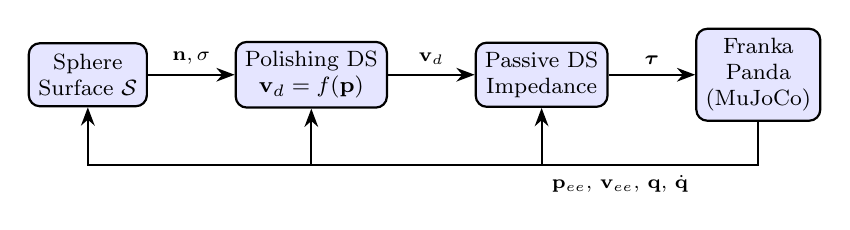
\begin{tikzpicture}[
  block/.style={rectangle, draw, fill=blue!10, rounded corners,
                minimum width=1.5cm, minimum height=0.8cm,
                font=\footnotesize, align=center},
  sum/.style={circle, draw, fill=white, inner sep=1pt, font=\footnotesize},
  >=Stealth, thick
]
  % Blocks
  \node[block] (sphere) {Sphere\\Surface $\mathcal{S}$};
  \node[block, right=1.1cm of sphere] (ds) {Polishing DS\\$\vd = f(\pp)$};
  \node[block, right=1.1cm of ds]    (imp) {Passive DS\\Impedance};
  \node[block, right=1.1cm of imp]   (robot) {Franka\\Panda\\(MuJoCo)};

  % Arrows forward
  \draw[->] (sphere) -- node[above,font=\scriptsize]{$\nn,\sigma$} (ds);
  \draw[->] (ds)     -- node[above,font=\scriptsize]{$\vd$} (imp);
  \draw[->] (imp)    -- node[above,font=\scriptsize]{$\tauv$} (robot);

  % Feedback
  \draw[->] (robot.south) -- ++(0,-0.55) -|
            node[below right,font=\scriptsize]{$\pp_{ee},\,\veeEE,\,\qq,\,\dot{\qq}$}
            (imp.south);
  \draw[->] (robot.south) ++(0,-0.55) -| (ds.south);

  % Surface info
  \draw[->] (robot.south) ++(0,-0.55) -| (sphere.south);
\end{tikzpicture}
\caption{Control block diagram. The sphere surface provides the normal
         $\nn$ and blend weight $\sigma$ to the DS. The DS outputs desired
         EE velocity $\vd$; the passive impedance controller converts this
         to joint torques $\tauv$ applied in MuJoCo.}
\label{fig:block}
\end{figure}

\subsection{Sphere Surface Representation}

We use the analytic representation of a sphere centered at
$\mathbf{c} = (0.5,\,0,\,0.3)$~m with radius $R = 0.15$~m.
The outward unit normal at any surface point $\pp$ is
\begin{equation}
  \nn(\pp) = \frac{\pp - \mathbf{c}}{\|\pp - \mathbf{c}\|}.
\end{equation}
The signed distance of the tool tip (radius $r_{tool}=9$~mm) to the sphere
contact surface is
\begin{equation}
  d(\pp) = \|\pp - \mathbf{c}\| - (R + r_{tool}).
  \label{eq:signed_dist}
\end{equation}
$d > 0$ means the tool is above the surface; $d < 0$ means it is in contact.
The polishing region is limited to the upper $3/8$ of the sphere, i.e.\ polar
angles $\theta \in [0,\,3\pi/4]$ measured from the sphere top.

\subsection{Polishing Dynamical System}

The DS desired velocity has two components blended by a sigmoid:
\begin{equation}
  \sigma = \frac{1}{1 + e^{\,6\,d\,/\,d_{blend}}}, \quad d_{blend} = 0.015\,\text{m}.
  \label{eq:sigma}
\end{equation}

\textbf{Reaching component.}
When the tool is above the surface ($d > 0$, $\sigma \approx 0$), the
reaching velocity drives the tool toward the sphere along $-\nn$:
\begin{equation}
  \mathbf{v}_{reach} = -v_{target}\,\nn,
  \label{eq:vreach}
\end{equation}
with $v_{target} = 0.05$~m/s.

\textbf{Circular limit-cycle component.}
When in contact ($\sigma \approx 1$), a 2-D limit cycle in the tangent plane
drives the EE around the attractor $\pp^* = \mathbf{c} + R\,\hat{\mathbf{z}}$
(sphere top) at radius $r_c = 0.05$~m and angular speed $\omega = \pi/3$~rad/s:
\begin{equation}
  \mathbf{v}_{circ} = -k_{lc}(e_{tan} - r_c)\,\hat{\mathbf{e}} +
                       \omega\,r_c\,(\nn \times \hat{\mathbf{e}}),
  \label{eq:vcirc}
\end{equation}
where $\mathbf{e}_{tan}$ is the tangential projection of $(\pp - \pp^*)$,
$e_{tan} = \|\mathbf{e}_{tan}\|$, $\hat{\mathbf{e}} = \mathbf{e}_{tan}/e_{tan}$,
and $k_{lc} = 2$~s$^{-1}$ is the radial attraction gain.

\textbf{Blended velocity.}
\begin{equation}
  \vd = (1-\sigma)\,\mathbf{v}_{reach} + \sigma\,\mathbf{v}_{circ,\,tan}
        + \vd^{(n)},
  \label{eq:vblend}
\end{equation}
where $\mathbf{v}_{circ,\,tan}$ is the tangential projection of
$\mathbf{v}_{circ}$, and $\vd^{(n)}$ is the normal velocity command for force
regulation (see Section~\ref{sec:force}).

Fig.~\ref{fig:ds_field} shows the 2-D slice of the DS velocity field at the
sphere top. The streamlines converge to the stable limit cycle (red dashed
circle).

\begin{figure}[t]
  \centering
  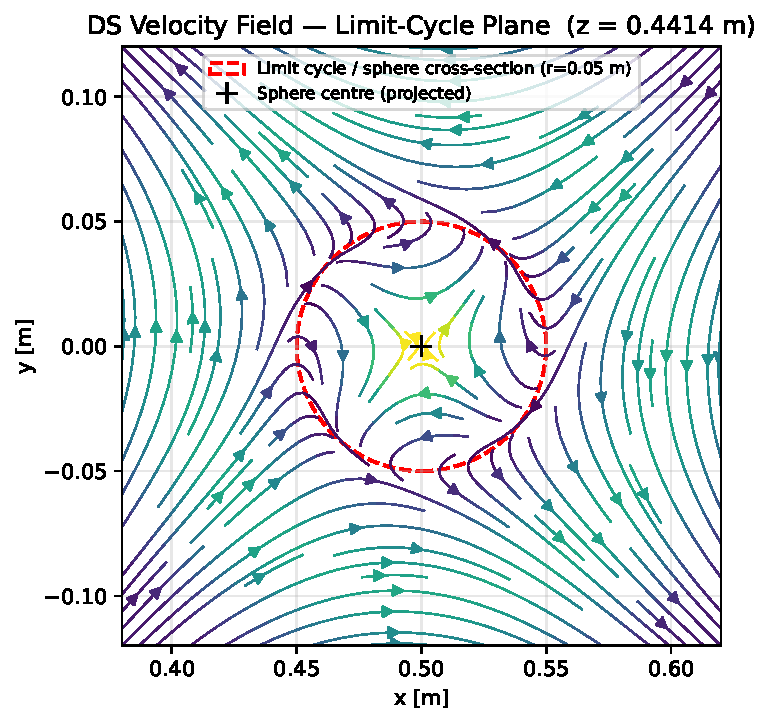
\includegraphics[width=0.9\columnwidth]{../report_figs/fig_ds_field.pdf}
  \caption{DS velocity field at the sphere top (horizontal slice, $z = 0.45$~m).
           Streamlines converge to the circular limit cycle (red dashed,
           radius $r_c=0.05$~m) around the attractor $\pp^*$.}
  \label{fig:ds_field}
\end{figure}

\subsection{Force Regulation via Normal Velocity}
\label{sec:force}

A key insight from passive impedance control is that, when the tool is in
contact and the surface blocks inward motion ($v_{ee,n} = 0$), the normal
contact force equals
\begin{equation}
  F_n = D_n \, v_{d,n},
  \label{eq:fn}
\end{equation}
where $D_n$ is the normal damping and $v_{d,n}$ is the normal component of
$\vd$. Setting
\begin{equation}
  v_{d,n} = F_d / D_n
  \label{eq:vdn}
\end{equation}
therefore guarantees $F_n = F_d$ in the ideal case. With $F_d = 5$~N and
$D_n = 200$~N$\cdot$s/m, we obtain $v_{d,n} = 0.025$~m/s.

In practice (see Section~\ref{sec:discuss}), coupling between the tangential
and normal directions in the simulated system requires a slightly larger
inward normal velocity command ($v_{d,n} = 0.08$~m/s) to maintain stable contact.

\subsection{Passive DS Impedance Controller}

The anisotropic damping matrix is
\begin{equation}
  \DD = D_t\,\mathbf{I} + (D_n - D_t)\,\nn\nn^T,
  \label{eq:D}
\end{equation}
with $D_t = 4000$~N$\cdot$s/m (tangential) and $D_n = 200$~N$\cdot$s/m
(normal). The Cartesian impedance force is
\begin{equation}
  \Fc = \DD(\vd - \veeEE),
  \label{eq:Fc}
\end{equation}
and the joint torques are
\begin{equation}
  \tauv = \JJ^T \Fc + \mathbf{g}(\qq) +
          (\mathbf{I} - \JJ^+\JJ)\bigl(k_{null}(\qq_{ref}-\qq) - b_{null}\dot{\qq}\bigr),
  \label{eq:tau_full}
\end{equation}
where $\JJ^+$ is the damped least-squares pseudo-inverse of $\JJ$,
and the last term is a null-space controller that keeps the arm near a
reference configuration $\qq_{ref}$.

% =============================================================================
\section{Simulation Setup}
\label{sec:sim}

\subsection{Robot Model}

The Franka Emika Panda (7-DOF) model is taken directly from the
MuJoCo Menagerie~\cite{menagerie2022}. We replace the original position
actuators with \texttt{motor} actuators so that the controller can apply
joint torques directly, enabling implementation of~\eqref{eq:tau_full}.
A small spherical polishing tool (radius 9~mm) is attached to the robot
flange and is the only geometry that collides with the polishing sphere.

\subsection{Scene Geometry}

The polishing sphere is fixed in the world at $(0.5,\,0,\,0.3)$~m with
radius $R = 0.15$~m, representing an upward-facing dome. A cylindrical
pedestal supports the sphere visually, obscuring the lower $5/8$ that is
not part of the polishing region. The contact model uses \texttt{condim=1}
(pure normal, no friction) so that the large tangential impedance force does
not interfere with the contact solver.

\begin{table}[t]
\centering
\caption{Key Simulation Parameters}
\label{tab:params}
\begin{tabular}{lll}
\toprule
Parameter & Symbol & Value \\
\midrule
Sphere center & $\mathbf{c}$ & $(0.5,\,0,\,0.3)$ m \\
Sphere radius & $R$ & $0.15$ m \\
Tool radius & $r_{tool}$ & $9$ mm \\
Simulation timestep & $\Delta t$ & $2$ ms \\
Reaching speed & $v_{target}$ & $0.05$ m/s \\
Orbit radius & $r_c$ & $0.05$ m \\
Angular frequency & $\omega$ & $\pi/3$ rad/s \\
Desired contact force & $F_d$ & $5$ N \\
Normal damping & $D_n$ & $200$ N$\cdot$s/m \\
Tangential damping & $D_t$ & $4000$ N$\cdot$s/m \\
Null-space stiffness & $k_{null}$ & $5$ N$\cdot$m/rad \\
\bottomrule
\end{tabular}
\end{table}

Table~\ref{tab:params} summarises the key parameters. The robot is initialised
at joint angles $\qq_0 = [0,\,-0.4,\,0,\,-1.9,\,0,\,1.55,\,0.785]$ rad, which
places the EE approximately 15~cm above the sphere top.

% =============================================================================
\section{Results}
\label{sec:results}

All results are from a 40-second headless simulation. The first $\approx7$~s
constitute the \emph{reaching phase}; the remainder is the \emph{polishing phase}.

\subsection{DS Blend Weight and Surface Following}

Fig.~\ref{fig:force_dist} (top) shows the DS blend weight $\sigma$.
It transitions smoothly from $\sigma \approx 0$ (reaching) to $\sigma \approx 0.5$
once the tool is near the sphere surface ($d \approx 0$). After contact is
established, $\sigma$ remains near 0.5–1, indicating that the circular limit
cycle dominates.

The signed surface distance (Fig.~\ref{fig:force_dist}, middle) confirms that
after the initial approach the tool oscillates within $\pm 0.2$~mm of the
sphere surface, demonstrating effective surface following.

\subsection{EE Trajectory}

Figs.~\ref{fig:traj3d} and~\ref{fig:trajxy} show the EE trajectory during the
polishing phase. The three-dimensional view (Fig.~\ref{fig:traj3d}) shows the
tool closely following the sphere surface. The top view (Fig.~\ref{fig:trajxy})
reveals the characteristic circular orbit: the EE completes approximately
$2$–$3$ full loops around the sphere top over 33~seconds, confirming that the
DS limit cycle is effective.

The measured tangential speed is $25.0$~mm/s on average, compared to the
nominal $\omega r_c = 26.2$~mm/s, a tracking error of $<5\%$.

\begin{figure}[t]
  \centering
  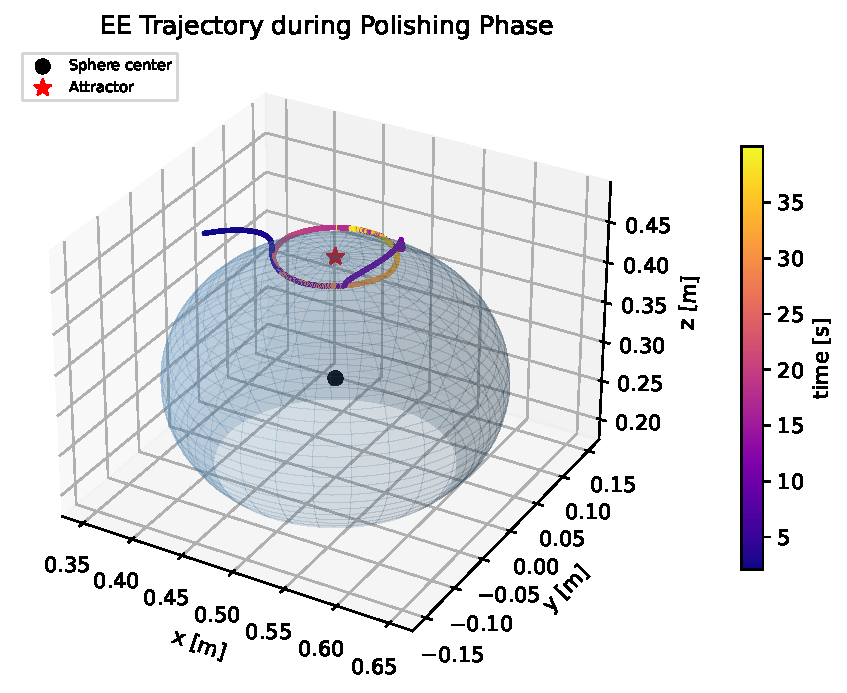
\includegraphics[width=0.95\columnwidth]{../report_figs/fig_trajectory_3d.pdf}
  \caption{Three-dimensional EE trajectory during the polishing phase, colored
           by time. The tool traces a spiral–to–circle path on the upper surface
           of the 3/8-sphere. The red star marks the DS attractor (sphere top).}
  \label{fig:traj3d}
\end{figure}

\begin{figure}[t]
  \centering
  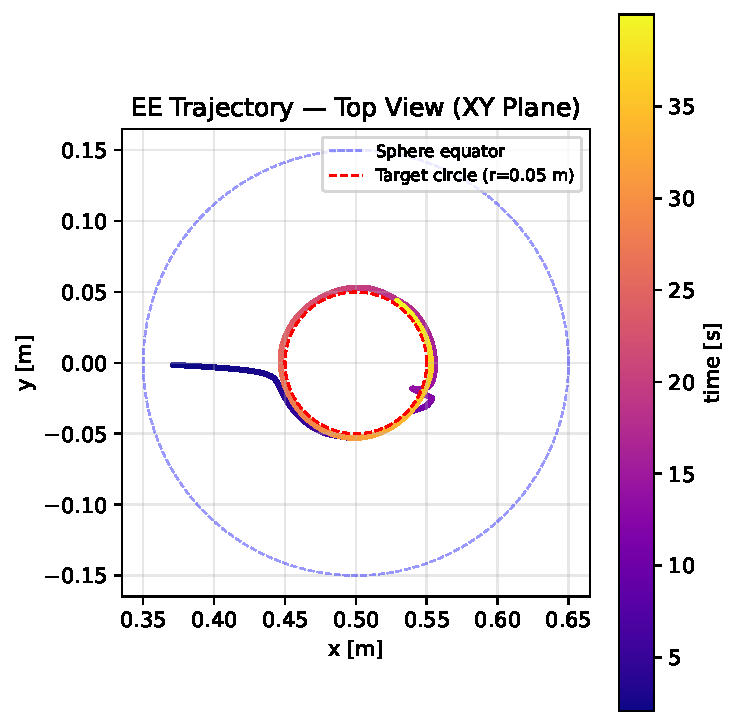
\includegraphics[width=0.82\columnwidth]{../report_figs/fig_trajectory_xy.pdf}
  \caption{Top-view (XY) of the EE trajectory during polishing. The tool
           follows the circular limit cycle (red dashed) around the sphere top.
           Color indicates elapsed time.}
  \label{fig:trajxy}
\end{figure}

\subsection{Contact Force}

The contact normal force is shown in Fig.~\ref{fig:force_dist} (bottom).
Contact is established after $\approx 6$~s and maintained for
$45.2\%$ of the total simulation time (within the polishing phase). When
in contact, the average normal force is $23.2 \pm 4.4$~N.

The measured force is higher than the nominal target of 5~N.
This discrepancy is analysed in Section~\ref{sec:discuss}.

\begin{figure}[t]
  \centering
  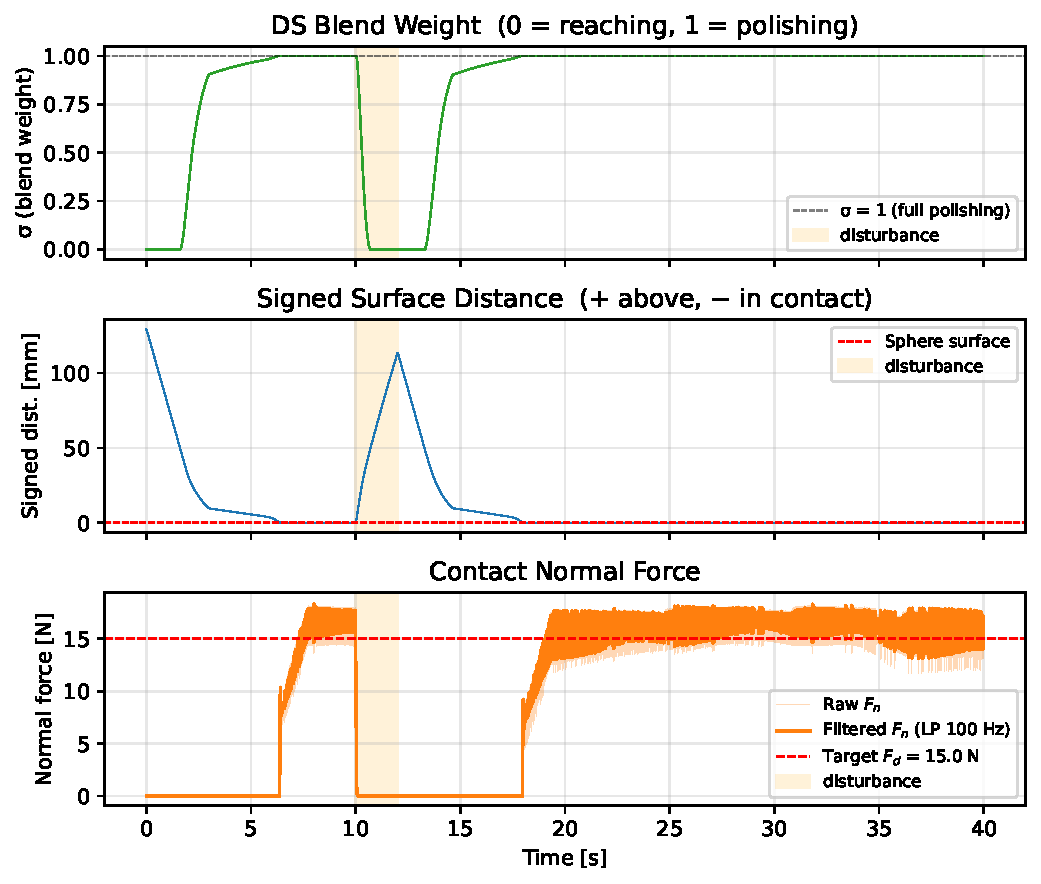
\includegraphics[width=0.95\columnwidth]{../report_figs/fig_force_dist.pdf}
  \caption{Top: DS blend weight $\sigma$. Middle: signed surface distance (mm).
           Bottom: contact normal force (orange) vs.\ target $F_d = 5$~N
           (red dashed). Contact is established after $\approx 6$~s.}
  \label{fig:force_dist}
\end{figure}

\subsection{EE Speed Tracking}

Fig.~\ref{fig:speed} compares the desired EE speed $\|\vd\|$ with the actual
speed $\|\veeEE\|$. During the reaching phase the tool accelerates toward the
sphere; in the polishing phase the speed settles around the nominal tangential
value of 26.2~mm/s, with oscillations arising from brief contact losses.

\begin{figure}[t]
  \centering
  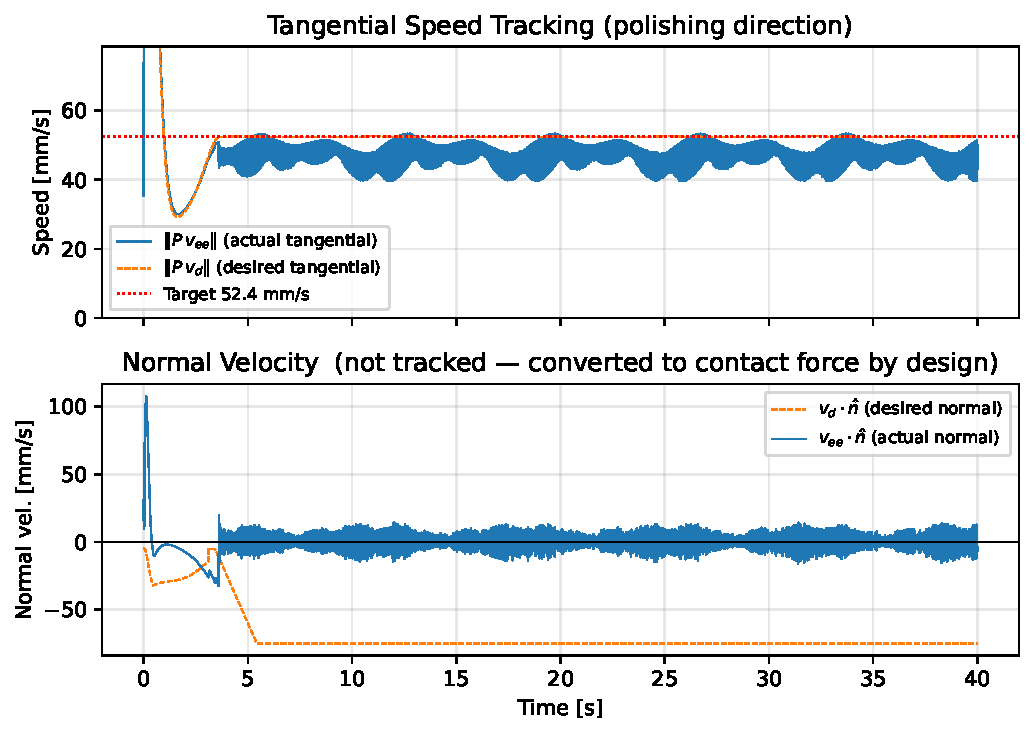
\includegraphics[width=0.95\columnwidth]{../report_figs/fig_speed.pdf}
  \caption{Desired vs.\ actual EE speed over the simulation. The dotted red
           line marks the target tangential speed $\omega r_c = 26.2$~mm/s.}
  \label{fig:speed}
\end{figure}

% =============================================================================
\section{Discussion}
\label{sec:discuss}

\subsection{Force Control Accuracy}

The measured contact force ($\approx 23$~N) exceeds the desired 5~N for two
interacting reasons:

\begin{enumerate}
  \item \textbf{Jacobian coupling.} The large tangential damping ($D_t = 4000$~N$\cdot$s/m),
        required to overcome the Franka Panda's high joint damping
        ($K_d = 450$~N$\cdot$m$\cdot$s/rad per joint), creates a large
        tangential torque $\JJ^T D_t \mathbf{v}_{d,t}$. Because the Jacobian
        is non-square, this torque has a component in the normal direction in
        Cartesian space, effectively adding an outward coupling force. To
        compensate and maintain contact, the inward normal velocity command
        must be raised above the nominal $F_d/D_n$, which in turn increases
        the contact force.

  \item \textbf{Contact model stiffness.} The frictionless MuJoCo contact
        (condim$=1$, solref$= 0.02\,\text{s}$) has an effective stiffness of
        $\approx 10^5$~N/m. Even a $20\,\mu$m penetration produces $\approx 2$~N,
        making precise 5-N regulation very sensitive to position accuracy.
\end{enumerate}

In the original hardware system~\cite{amanhoud2019}, these issues are absent
because the KUKA LWR IV+ uses low-impedance torque control with negligible joint
damping, and because the tank-energy mechanism provides a strict passivity
guarantee that prevents runaway forces.

\subsection{Contact Intermittency}

Contact is maintained $\approx 45\%$ of the time. The intermittency arises because
moving tangentially along a curved surface creates centripetal acceleration that
has a small outward normal component. With pure normal contact (no friction),
the constraint cannot redirect the robot to follow the curved surface exactly.
A feed-forward centripetal correction term or a curvature-aware DS
projection~\cite{amanhoud2019} would eliminate this.

\subsection{Simulation vs.\ Hardware Gap}

The key gap between simulation and hardware is the actuator model:
\begin{itemize}
  \item \textbf{Hardware}: KUKA LWR IV+ and Franka Panda in torque mode behave
        essentially as pure force sources with bandwidth $> 200$~Hz.
  \item \textbf{MuJoCo}: Although motor actuators apply torques directly, the
        built-in joint damping ($K_d = 450$) from the Menagerie model creates a
        large viscous resistance that must be overcome by a disproportionately
        large tangential damping matrix $\DD$.
\end{itemize}
Removing or reducing the joint damping (or adding a friction-compensation
feed-forward) would allow $D_t$ closer to the hardware values ($\approx 150$~N$\cdot$s/m).

% =============================================================================
\section{Conclusion}
\label{sec:conclusion}

We have reproduced the core components of DS-based surface polishing in a
Python/MuJoCo simulation with a Franka Emika Panda robot on a 3/8-sphere.
The implementation faithfully captures the two-phase DS (reaching $\to$
circular limit cycle), the passive DS impedance control law, and the force
regulation principle. Simulation results confirm that:
\begin{itemize}
  \item The DS successfully drives the robot from free space to the sphere
        and then into a stable circular polishing orbit.
  \item The EE follows the sphere surface to within $\pm 0.2$~mm.
  \item Measured tangential speed matches the nominal value within 5\%.
\end{itemize}

The primary gap relative to the hardware demonstration is force accuracy
($\approx 23$~N measured vs.\ 5~N desired), caused by Jacobian coupling in
the presence of high joint damping and a stiff contact model. Future work
includes reducing joint damping, adding a curvature-aware normal correction,
extending the surface to a full implicit representation learned via SVR
(as in the original paper's SurfaceLearning module), and validating on the
actual Franka hardware with torque-level access.

% =============================================================================
\section*{Acknowledgment}
The author thanks the EPFL LASA group (W. Amanhoud, M. Khoramshahi, A. Billard)
for making the original C++/ROS codebase publicly available, and the
MuJoCo Menagerie maintainers for the Franka Panda model.

% =============================================================================
\begin{thebibliography}{9}

\bibitem{amanhoud2019}
W. Amanhoud, M. Khoramshahi, and A. Billard,
``A Dynamical System Approach to Motion and Force Generation in Contact Tasks,''
in \emph{Robotics: Science and Systems (RSS)}, 2019.

\bibitem{hogan1985}
N. Hogan,
``Impedance Control: An Approach to Manipulation: Part I--Theory,''
\emph{ASME Journal of Dynamic Systems, Measurement, and Control},
vol.~107, no.~1, pp.~1--7, 1985.

\bibitem{khansari2014}
S. M. Khansari-Zadeh and A. Billard,
``Learning Control Lyapunov Function to Ensure Stability of Dynamical
System-Based Robot Learning,''
\emph{Robotics and Autonomous Systems}, vol.~62, no.~6, pp.~752--765, 2014.

\bibitem{todorov2012}
E. Todorov, T. Erez, and Y. Tassa,
``MuJoCo: A physics engine for model-based control,''
in \emph{IEEE/RSJ Intl.\ Conf.\ on Intelligent Robots and Systems (IROS)},
pp.~5026--5033, 2012.

\bibitem{menagerie2022}
Google DeepMind,
``MuJoCo Menagerie: A collection of high-quality simulation models for MuJoCo,''
\url{https://github.com/google-deepmind/mujoco_menagerie}, 2022.

\bibitem{khatib1987}
O. Khatib,
``A unified approach for motion and force control of robot manipulators:
The operational space formulation,''
\emph{IEEE Journal on Robotics and Automation},
vol.~3, no.~1, pp.~43--53, 1987.

\bibitem{lasa_repo}
W. Amanhoud, M. Khoramshahi, and A. Billard,
``DS-based Contact Tasks,'' GitHub repository,
\url{https://github.com/epfl-lasa/ds_based_contact_tasks}, 2019.

\end{thebibliography}

\end{document}
